\section{Auswertung}
\label{sec:auswertung}

Im Anschluss werden die aufgenommenen Messwerte ausgewertet.

\subsection{Energiekalibration und Bestimmung der Vollenergienachweiswahrscheinlichkeit.}
\label{sec:auswertung1}

Das aufgenommene Spektrum der Eu-152 Quelle ist in der Abbildung \ref{fig:plot1}
dargestellt. Die Anzahl der Impulse wurden für eine bessere Darstellbarkeit logarithmisch abgebildet. 

\begin{figure}[H]
    \centering
    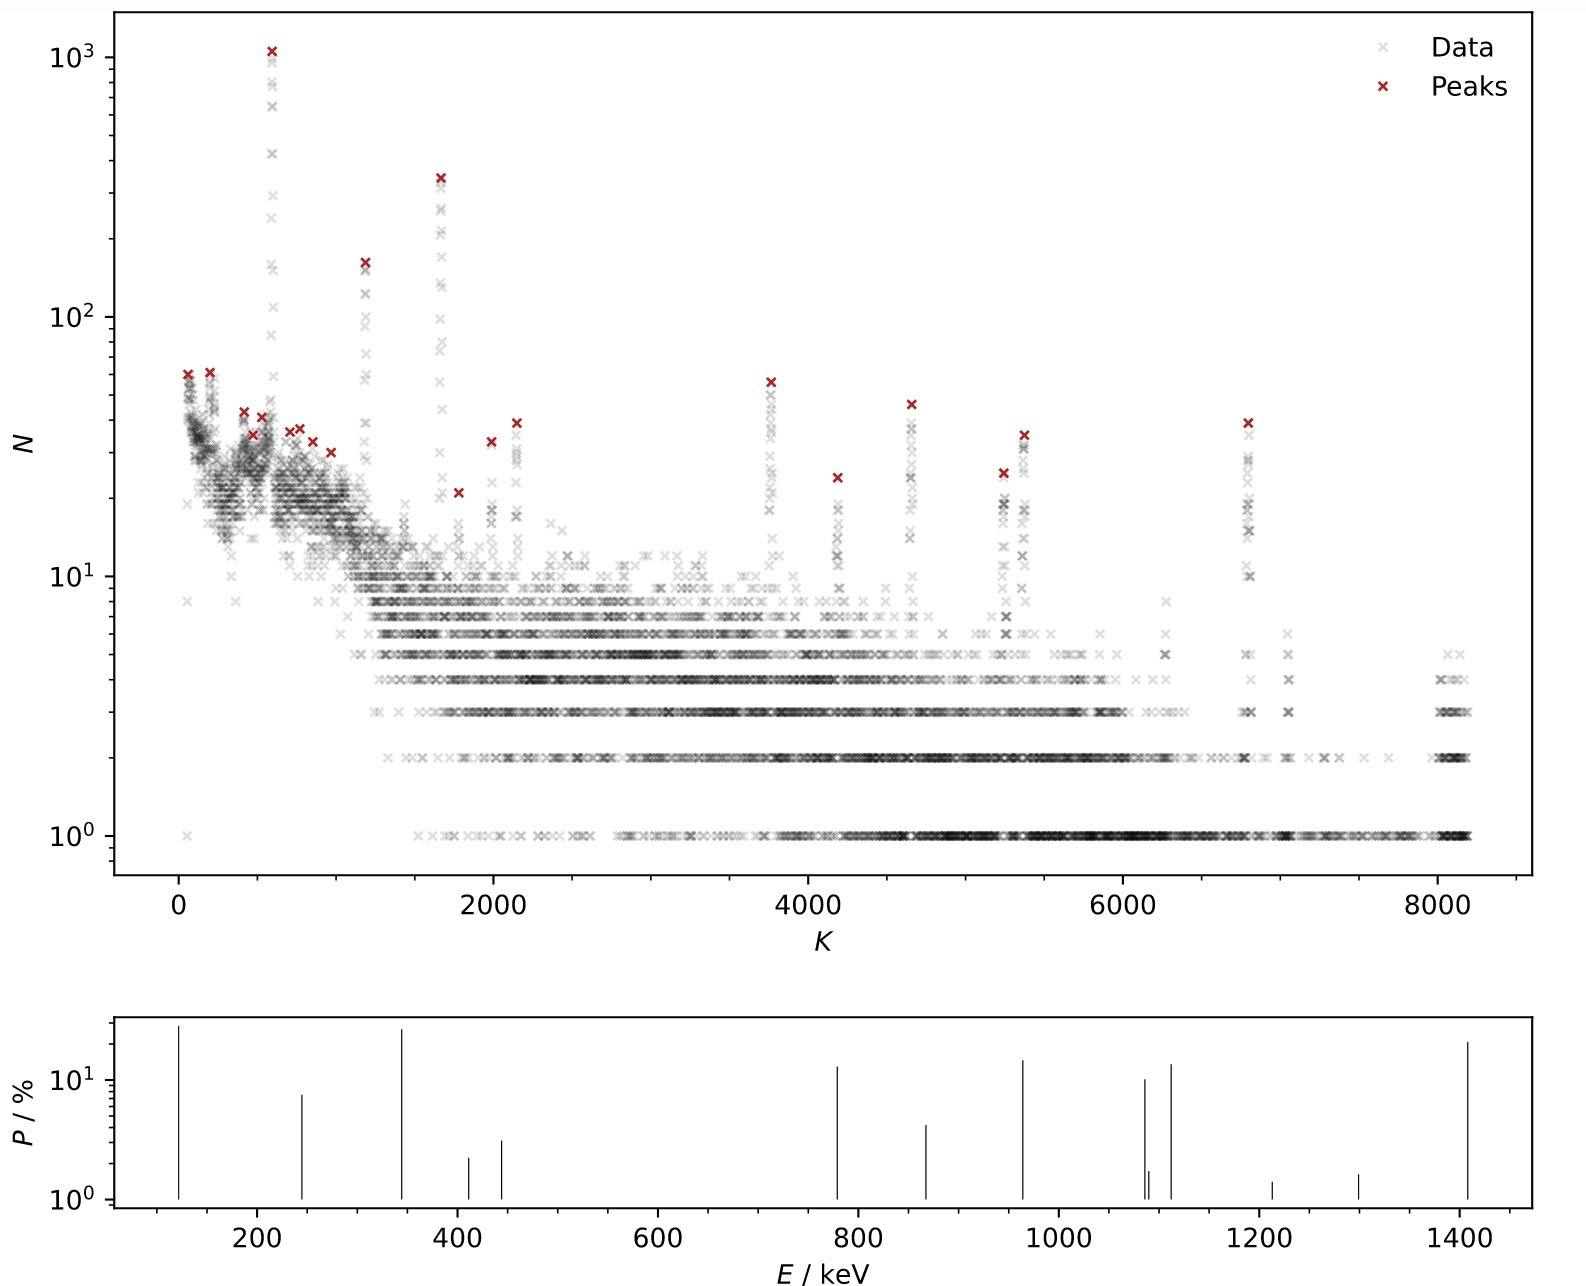
\includegraphics[width=0.9\textwidth]{content/plots/plot1.jpg}
   \caption{Gammaspektrum des Eu-152 Strahlers.}
    \label{fig:plot1}
\end{figure}

Die Photopeaks werden mit dem SciPy Paket find-peaks ermittelt und rot markiert.
Unter dem Spektrum befinden sich die Emissionsenergien des Gammastrahlers, welche zum Abgleichen verwendet werden.
Die Emissionsenergien von Eu-152 sind in der Abbildung \ref{fig:euE} gegeben.

\begin{figure}[H]
    \centering
    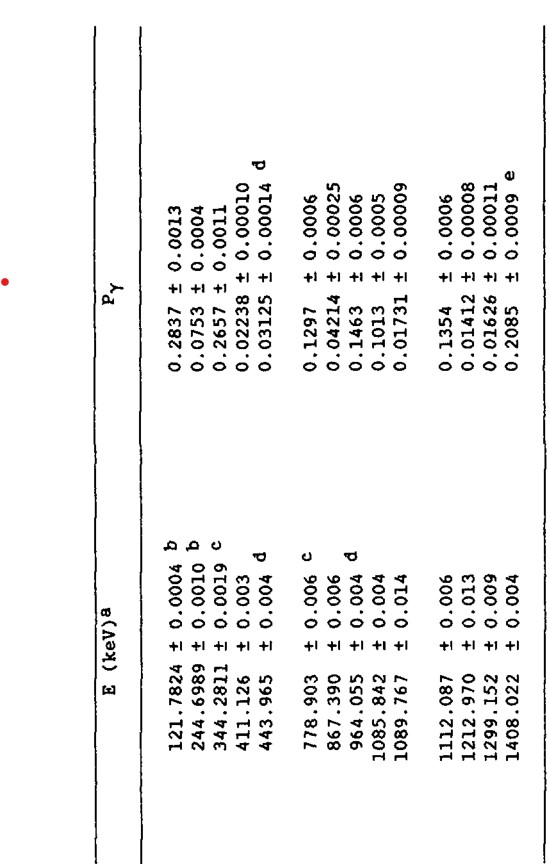
\includegraphics[angle=270,width=0.6\textwidth]{content/grafik/euenergien.jpg}
    \caption{Die Emissionsenergien von Eu-152. \cite{Kalibration}}
    \label{fig:euE}
\end{figure}

Nun werden die zugeordneten Emissionsenergien gegen die Kanäle aufgetragen.
Anschließend wird eine lineare Ausgleichsgerade der Form 
\begin{equation*}
    a \cdot K + b
\end{equation*}
an die Werte angelegt. $K$ bezeichnet dabei die Kanalnummer.
Die Ausgleichsgerade ist in der Abbildung \ref{fig:plot2}
zu sehen.

\begin{figure}[H]
    \centering
    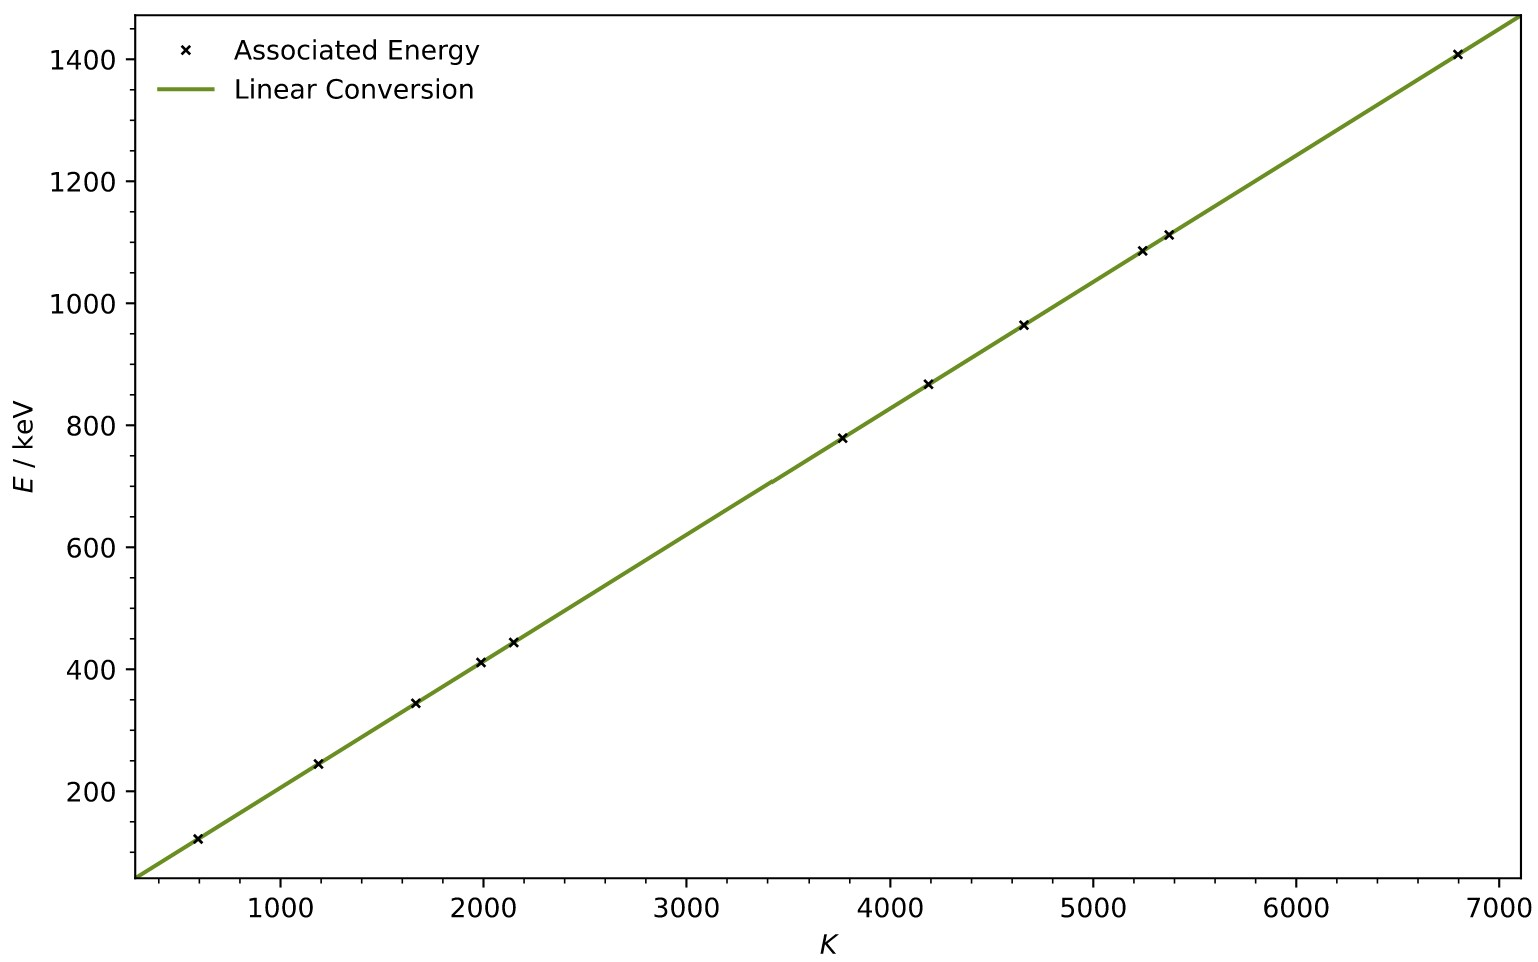
\includegraphics[width=0.8\textwidth]{content/plots/plot2}
    \caption{Ausgleichsrechnung der Energiekalibration.}
    \label{fig:plot2}
\end{figure}

Für die Parameter ergeben sich die Werte
\begin{align*}
    a   &= \qty{0.2073+-0.0001}{\kilo\eV} \\
    b   &= \qty{-1.3399 +- 0.2191}{\kilo\eV}.
\end{align*}

Für die Energiekalibration ergibt sich demnach
\begin{equation*}
    E\left(K\right) = \qty{0.2073+-0.0001}{\kilo\eV} \cdot K + \qty{-1.3399 +- 0.2191}{\kilo\eV}.
\end{equation*}

Zur Verdeutlichung der Zuordnung der Emissionswahrscheinlichkeiten wurde das Spektrum von Eu-152 mit der Energieskala erneut erstellt und
wird in der Abbildung \ref{fig:plot3}
abgebildet.

\begin{figure}[H]
    \centering
    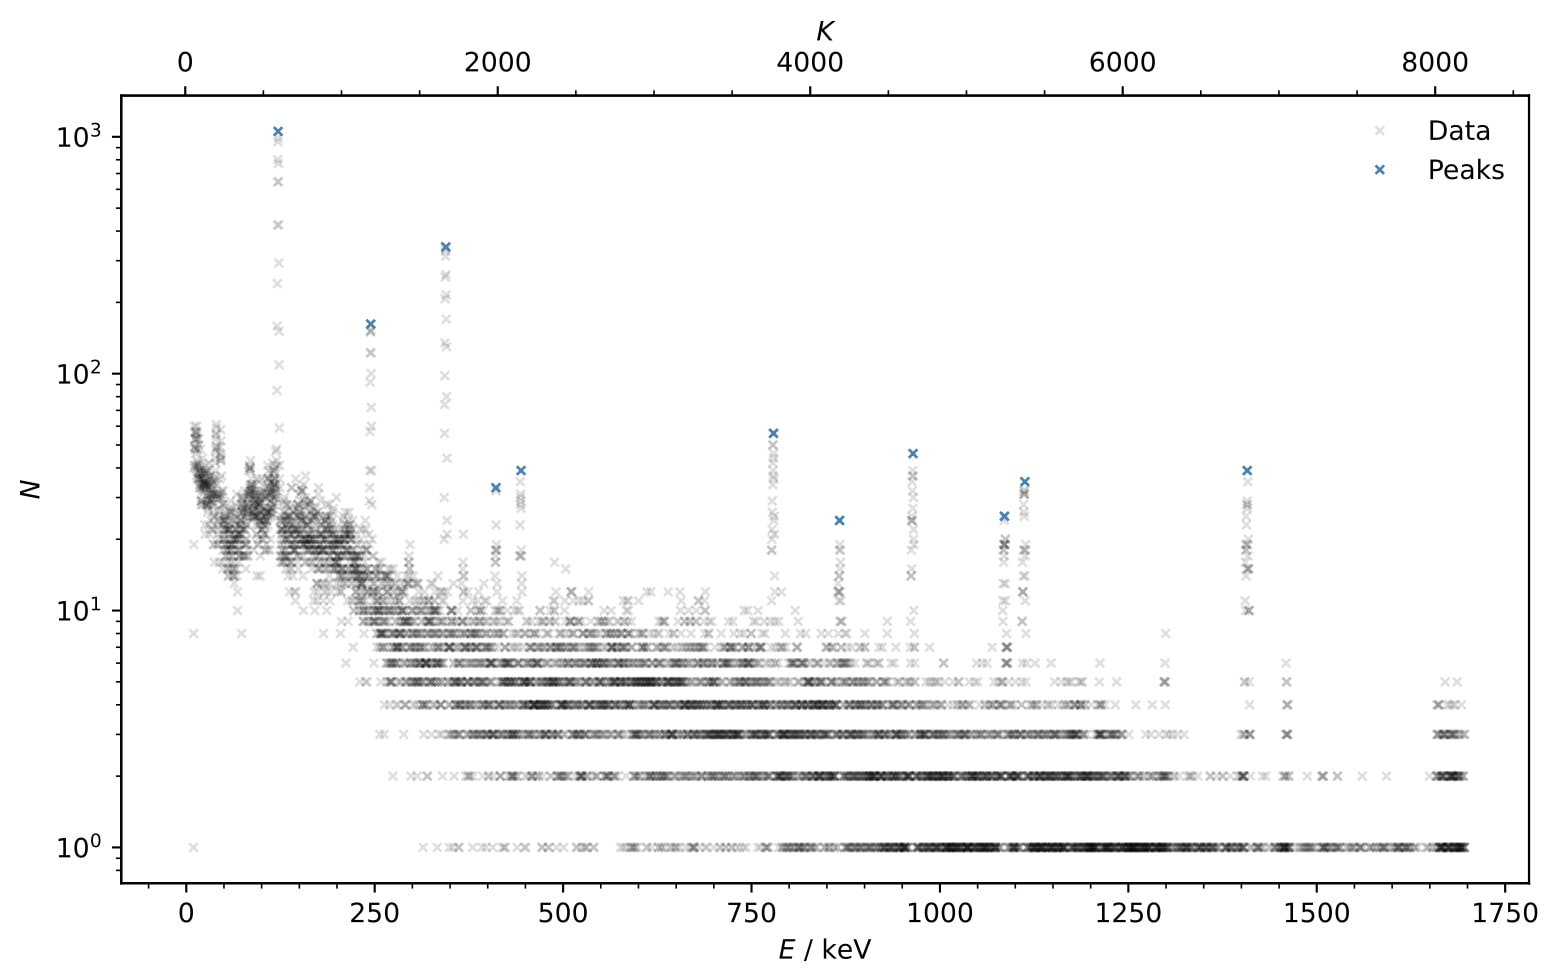
\includegraphics[width=0.8\textwidth]{content/plots/plot3}
   \caption{Gammaspektrum des Eu-152 Strahlers mit zusätzlicher Energieskala.}
   \label{fig:plot3}
\end{figure}